\documentclass[10pt,twocolumn]{article}
\setlength{\columnsep}{45pt}
% Language setting
% Replace `english' with e.g. `spanish' to change the document language
\usepackage[italian]{babel}

% Set page size and margins
% Replace `letterpaper' with `a4paper' for UK/EU standard size
\usepackage[letterpaper,top=2cm,bottom=2cm,left=3cm,right=3cm,marginparwidth=1.75cm]{geometry}

% Useful packages

\usepackage[style=authoryear-comp]{biblatex}
\usepackage{filecontents}
\usepackage{amsmath}
\usepackage{graphicx}
\usepackage{amssymb}
\usepackage[colorlinks=true, allcolors=blue]{hyperref}
\usepackage[most]{tcolorbox}
\newcommand{\definition}[1]{\colorbox{SkyBlue!30}{#1}}
\hypersetup{ 
     colorlinks=true, 
     linkcolor=black, 
     filecolor=black, 
     citecolor = black,       
     urlcolor=blue, 
     } 
\begin{filecontents*}{database.bib}
@article{gplv3,
  title        = {MIT License},
  version      = {Copyright (c) 2023 Leonardo Marro},
  journal    = {Permission is hereby granted, free of charge, to any person obtaining a copy
of this file and associated documentation files (the "File"), to deal
in the File without restriction, including without limitation the rights
to use, copy, modify, merge, publish, distribute, sublicense, and/or sell
copies of the File, and to permit persons to whom the File is
furnished to do so, subject to the following conditions:},
text2 = {The above copyright notice and this permission notice shall be included in all
copies or substantial portions of the Software.},
text3 = {THE FILE IS PROVIDED "AS IS", WITHOUT WARRANTY OF ANY KIND, EXPRESS OR
IMPLIED, INCLUDING BUT NOT LIMITED TO THE WARRANTIES OF MERCHANTABILITY,
FITNESS FOR A PARTICULAR PURPOSE AND NONINFRINGEMENT. IN NO EVENT SHALL THE
AUTHORS OR COPYRIGHT HOLDERS BE LIABLE FOR ANY CLAIM, DAMAGES OR OTHER
LIABILITY, WHETHER IN AN ACTION OF CONTRACT, TORT OR OTHERWISE, ARISING FROM,
OUT OF OR IN CONNECTION WITH THE SOFTWARE OR THE USE OR OTHER DEALINGS IN THE
SOFTWARE.},
  
  pagination   = {section},

  date         = {2023-03-02}
  }
\end{filecontents*}
\usepackage[T1]{fontenc}
\usepackage[
    type={CC},
    modifier={by-nc-sa},
    version={3.0},
]{doclicense}
\bibliography{database.bib}
\title{Basi di Dati}
\author{Leonardo Marro}

\begin{document}


\twocolumn[{\centering{\Huge Basi di Dati \par}\vspace{3ex}
        {\large Leonardo Marro \par}\vspace{3ex}
	\today\par\vspace{4ex}{\small \fbox{\doclicenseThis} \par}\vspace{2ex}}]
 
 \hypertarget{home}{ }
 \tableofcontents
 \clearpage
\part{Introduzione Alla Teoria}

\section{Sistema Informativo}

Un Sistema Informativo è un componente di un'organizzazione che gestisce le informazioni di interesse (utili).

[Imm 1]
Gestione delle info:
\begin{itemize}
    \item Raccolta, acquisizione;
    \item Archiviazione;
    \item Elaborazione;
    \item Distribuzione.
\end{itemize}
Le informazioni vengono rappresentate attraverso i \textbf{Dati}.
\newline
Informazioni: Dati che assumono uno specifico significato in un determinato contesto. (Ovvero dati interpretati o correlati).


\section{Basi di Dati}
\begin{itemize}
    \item Accezione metodologica, generica: \textbf{Insieme Organizzato} di un ente pubblico o privato. 
    \item Accezione specifica, metodologica e tecnologica:
    \begin{itemize}
        \item insieme di dati gestito da un DBMS (DataBase Management System).
    \end{itemize}
\end{itemize}
Una \textbf{base di dati} è insieme di dati atomici strutturati e persistenti, raggruppati in \textbf{insiemi omogenei in relazione tra loro} organizzati con la minima ridondanza per essere utilizzati da applicazioni diverse in modo sicuro e controllato.
\subsection{Caratteristiche di Basi di Dati}
\begin{itemize}
    \item Condivise
    \begin{itemize}
        \item Organizzazioni divise in settori con diverse attività.
        \item Ciascun settore/attività ha un sottosistema informativo (non per forza totalmente separati)
    \end{itemize}
    [imm2]
\end{itemize}
Una base di dati è una risorsa integrata condivisa tra applicazioni con le seguenti conseguenze:
\begin{itemize}
    \item Attività svolte da utenti che usano dati condivisi $->$ vengono richiesti \textbf{meccanismi di autorizzazione}.
    \item Accessi da diversi soggetti in unisono $->$ vengono richiesti dei controlli della \textbf{concorrenza}.
\end{itemize}
Di base il rapporto costo$/$ n°settori è esponenziale, questo comporta un eventuale \textbf{collasso}.
\newline \textbf{Criticità e costi}:
\begin{itemize}
    \item Eterogeneità dei sistemi: fornitori e tecnologie.
    \item Difficoltà nell'interscambio di dati incompatibili.
    \item Ridondanza e incoerenza delle informazioni.
    \item Assenza di una visione unitaria (Programmatori differenti).
\end{itemize}
Si usa allora lo sviluppo integrato per migliorare l'efficienza.
\subsection{Sviluppo Integrato}
\begin{enumerate}
    \item Data la struttura organizzata si esegue un'\textbf{analisi} attenta del sistema informativo (come funziona).
    \item Definiti schema e dati e info di interesse, si sviluppa l'applicazione.
    \item L'app si interfaccia attraverso il DBMS in base alle sue esigenze.
\end{enumerate}
\begin{align}
    \text{\textcolor{red}{Prima i Dati, Poi le Applicazioni!}}
\end{align}

\section{Il modello relazionale}
[tabella da copiare (ospedale)]
\newline
Il termine tabella è errato, sono chiamate \textbf{relazioni}.
Ogni relazione contiene il suo \textbf{nome}, degli \textbf{attributi} (o campi o proprietà)(intestazioni delle singole colonne), l'insieme di tutti gli attributi rappresenta lo \textbf{schema} della relazione.\newline All'interno della tabella si trovano \textbf{tupla}(o n-upla o record) che rappresentano occorrenze dei medici (in questo esempio) descritti dagli attributi, l'insieme delle tuple si chiama \textbf{istanza} della relazione, in fine abbiamo il singolo \textbf{dato} (il quale ottiene un significato grazie alla correlazione degli attributi).  \newline In una relazione può essere presente un attributo sottolineato, chiamato \textbf{attributo identificatore} della relazione, nel nostro esempio attraverso quel dato possiamo identificare i singoli medici. \newline Attraverso l'attributo Primario$/$MATR possiamo correlare le relazioni. 

\subsection{Relazione}
Una relazione è definita:
\begin{itemize}
    \item da uno \textbf{schema} della relazione
    \item dalla \textbf{istanza} della relazione (o stato)
\end{itemize}
L'\textbf{attributo} di una relazione è definito come una coppia $A_i:T_i$
\begin{itemize}
    \item $T_i$ è il tipo dell'attributo;
    \item $A_i$ è il nome dell'attributo.
\end{itemize}
\begin{itemize}
    \item Tipi standard (o default):
    \begin{itemize}
        \item Integer, Real, String...
    \end{itemize}
    \item Tipi utente (definiti dall'utente sotto certe restrizioni); non si possono raggruppare diversi tipi.
\end{itemize}
Tipo $T_i$ caratterizzato da:
\begin{itemize}
    \item $T_i$ nome identificativo del tipo;
    \item $D_i$ dominio di valori;
    \item collezione di \textbf{operazioni} che agiscono su $D_i$ ($+,-,*,/$);
    \item operazioni di \textbf{confronto} su $D_i$ ($<, >, \leq, \geq$).
\end{itemize}
\subsection{Dominio di un attributo}
Un tipo è \textbf{sempre associato} ad un \textcolor{red}{dominio}. Questo avviene attraverso la funzione \textbf{\textit{dom}} che associa $A_i$ con il suo dominio $D_i$.
\[D_i = dom(A_i)\]
\subsection{Valore nullo}
Se alla creazione di un elemento non conosco un suo dato, esiste un valore speciale chiamato \textbf{valore nullo} o \textbf{NULL} con la seguente proprietà: \[\forall T_i, \text{NULL} \in D_i\] ovvero il valore NULL appartiene al dominio $D_i$ di qualsiasi tipo $T_i$.
\subsection{Schema di una relazione}
Lo schema di una relazione è un insieme di attributi con la seguente notazione: \[A_1 : T_1 ,....., A_n : T_n\] Sono insiemi di attributi tutti con \textbf{nomi distinti}; possono avere tipi uguali all'interno della stessa relazione, mentre l'ordine degli attributi è \textbf{irrilevante} (nella definizione formale di Codd).
\subsection{Schemi con nomi}
Lo schema di una relazione \textbf{con nome} ha la seguente notazione: \[ R(A_1:T_1 ,...., A_n:T_n)\] dove R è un generico nome. In certi casi il nome si può sotto intendere, ma nei DBMS è \textbf{obbligatorio specificarlo}. Esempio:\[\text{Pazienti}(\text{COD, Cognome, Nome....})\]
\subsubsection{Notazione Generale}
Definendo l'insieme di attributi A, posso usare la notazione $R(A)$ per indicare l'insieme degli attributi per sintetizzare la rappresentazione, dove R è il nome dello schema.
\subsection{Grado di una relazione}
La \textbf{cardinalità} di $|A|$ di uno schema è il n° degli attributi dello schema A. L'insieme di attributi di uno schema di una relazione è sempre un insieme \textbf{non vuoto}, ovvero $|A| > 1$.
\subsection{Istanza (o stato) di una relazione}
Dato uno schema A, l'\textbf{istanza} o \textbf{stato} r di una relazione è un insieme di tuple $<v_1,...,v_n$ aventi la proprietà: \[\forall i, v_i \in dom (A_i)\]
\subsection{Cardinalità di una relazione}
La cardinalità $|r|$ di una relazione è il numero di tuple$\in$ r, detta \textbf{cardinalità di una relazione}. Con il simbolo t, si indica la singola tupla. 
\subsection{Notazioni ibride}
Utilizziamo lettere maiuscole per indicare le relazione, mentre uso le minuscole per indicare le istanze delle relazioni.
\subsection{Notazione tabellare}
[imm tabella]
\subsection{Relazione (notazione)}
La relazione è definita da una coppia \[<R,r>\] dove R è lo schema e R è l'istanza.
\subsubsection{Tupla}
Data una relazione r, per indicare una singola tuple, si usa: \[t=<v_1,...,v_n>\], quindi $t\in r(A_1,...,A_n)$.
\subsubsection{Valori di una tupla}
Per indicare il valore di una tupla t si usa la notazione $t[A_i]$, quindi $t[A_i]=v_i$. Ricordarsi che l'ordine non è importante. Esiste anche la dot-notation ($t.A$) in aggiunta alla notazione standard.
\section{Relazione matematica e Relazione di Codd}
In matematica $A\times B$ è diverso da $B\times A$, per cui le relazioni sono dipendenti dall'ordine, questo si oppone al modello relazionale il quale considera l'ordine irrilevante. In oltre in matematica una relazione è è un sottoinsieme di un prodotto cartesiano: $s \subset \{ dom(A_1)\times dom(A_2) \times ... \}$.  \newline Una \textbf{funzione totale} $f:X \rightarrow Y$ può essere vista come un insieme di tuple.\newline Il dominio sono gli attributi e i codominio sono i valori degli attributi corrispondenti. Avremo la funzione $t:\{ A_1,A_2,....,A_n\} \rightarrow D $ con $D = \{ dom(A_1)\cup dom(A_2) \cup ...\}$.\newline Una tupla, in quanto una funzione, si può anche rappresentare anche sotto forma di tabella: [imm tabella]. \newline \textbf{N.B.} Tutte le tuple (quindi anche funzioni) $t_i$ sono \textbf{tutte distinte}, in quanto due tuple identiche non possono esistere. \newline Una tupla t si dice \textbf{compatibile} con lo schema A se: \begin{itemize}
    \item t è \textbf{funzione totale} su A;
    \item ogni valore di t$\in$D;
    \item vale il vincolo $\forall A_i, t[A_i] \in dom(A_i)$
\end{itemize}
\section{Vincoli}
\subsection{Vincoli locali}
I \textbf{vincoli locali} sono caratterizzazioni dei valori che le tuple posso ottenere per farle rispettare la realtà da rappresentare. Si possono considerare come delle restrizioni sui valori delle tuple.
\subsubsection{Vincolo locale di dominio}
Per ogni attributo ho un \textbf{insieme ben definito} di valori possibili, quindi qualsiasi valore $v_i$ del dominio D è \textbf{atomico}(singolo carattere, singola stringa, etc.), se invece il valore dell'attributo è una relazione, non può essere atomico. \textbf{NON PERMESSO}.
\subsection{Vincoli su valori nulli}
Un vincolo NOT NULL è soddisfatto se il valore bersaglio $\forall t \in r,$  il valore $t[A_i]$ \textbf{non è nullo}.
\subsection{Altri vincoli}
Possiamo introdurre \textbf{restrizioni sui domini} (una persona non può avere più di 120 anni) per obbligare i valori ad avere un certo senso, oppure introduciamo \textbf{confronti sui domini} (la data di inizio deve essere antecedente alla data di conclusione).
\subsection{Vincolo di identificazione}
Questo vincolo viene applicato attraverso il vincolo di \textbf{chiave relazionale}, indica il contesto applicativo (ad esempio la matricola di uno studente), questi vincoli possono essere composti da \textbf{più valori}. Nelle relazioni di Codd tutti gli elementi dell'istanza devono essere distinti tra di loro.
\subsection{Superchiave}
Data una relazione $r(A)$, un sottoinsieme di attributi $sk \subseteq A$ è una \textbf{superchiave} se: \[ \forall i,j (t_i[sk] = t_j[sk]) \rightarrow (t_i[A] = t_j[A])\] 
\subsection{Verifica dell'implicazione}
\[\alpha \rightarrow \beta \text{ equivalente a} (\lnot \alpha \lor \beta) \]
Verifico l'unicità con i diversi valori della stessa tabella sotto lo stesso parametro, un dato deve essere \textbf{SOLO uguale a se stessa}; se questa condizione non è valida per almeno una tupla, allora la tupla \textbf{non è superchiave}.
\subsubsection{Da quantificazione universale ad esistenziale}
\[ \alpha \rightarrow \beta \equiv (\neg \alpha \lor \beta)\]
negandola
\[\neg (\alpha \rightarrow \beta) \equiv \neg(\neg \alpha \lor \beta)\] da cui \[ \nexists i,j (t_i[sk]=t_j[sk]) \rightarrow (t_i \neq t_j)\]
\subsection{Chiave candidata}
$k \subseteq A$ si dice \textbf{chiave candidata} se k è \textbf{superchiave} di R e k è \textbf{superchiave minimale}, ovvero una superchiave il cui sottoinsieme non è a sua volta una superchiave.
\subsubsection{Proprietà delle superchiavi}
Se sk è una superchiave allora $sk \subseteq w \subseteq A$ è una \textbf{superchiave} per cui A è necessariamente una superchiave e di conseguenza A contiene almeno una chiave candidata.
Sarà a discrezione del progettista scegliere una sola \textbf{Chiave principale} (o primaria). Tutti gli attributi di una chiave principale devono essere \textbf{NON NULLI}, mentre una chiave candidata può averne.
\subsubsection{Correttezza di una relazione}
Un'istanza di una relazione $r(A)$ è corretta se per ogni tupla $t \in r$ è compatibile con lo schema A e sono soddisfatti tutti i vincoli locali.
\section{Relazione in prima forma normale}
Una relazione si dice in \textbf{prima forma normale} quando tutti gli attributi hanno domini di valori atomici. Verrà approfondito nell'argomento della \textbf{normalizzazione}. Questo serve a verificare la compatibilità della tupla e a controllare che gli eventuali valori non siano nulli.
\subsection{Schema di una basi di dati}
Lo schema di una base di dati è un insieme di schemi con nome \[ S = \{ R_1, R_2,....,R_n\}\]
identificati dalle seguenti proprietà:\begin{itemize}
    \item I nomi sono distinti;
    \item Ogni schema possiede i rispettivi vincoli locali;
    \item Ogni relazione $R_i$ possiede una chiave principale.
\end{itemize}
Ogni relazione va successivamente definita.
\subsection{Vincoli globali su S}
Su ogni relazione R si può definire un vincolo globale \textbf{interrelazionali} su uno schema S, il più importante è il \textbf{vincolo di integrità referenziale} (foreign key).
\subsubsection{Vincolo di integrità referenziale}
Sotto esempio: Se in RICOVERI c'è una tupla $t.[PAZ]=X$ allora necessariamente in PAZIENTI dovrà esistere una tupla $t.[COD]=X$. Questo criterio non per forza deve essere inverso. 


Definizione:\newline
\textit{\large Considerando la relazione $R_h (PK,..)$ dove PK è l'insieme di attributi della chiave principale e la relazione $R_S(...B...)$ dove B sono un insieme di attributi, \textbf{Esiste un vincolo di integrità referenziale} di B rispetto a $R_h$ se}: \[\forall t_i (t_i \in r(R_j))\rightarrow \exists t_j (t_j \in r(R_h)) \land (t_i[B] = t_j[PK])\]
Ovviamente i vincoli devono essere compatibili.
\subsection{Stato o istanza di una base di dati}
Lo stato di una base di dati è definito come \[ DB= (<R_1 , r_1>,...,<R_n,r_n)\]
dove ogni $r_i$ deve essere corretta e devono soddisfare i vincoli globali.

Si può concludere l'argomento specificando che il modello relazionale è un \textbf{modello di dati orientato ai valori}, mentre in altri modello le corrispondenze avvengono attraverso riferimenti.
\clearpage
\part{Algebra Relazionale}
\section{Modello interrogazione di Codd}
Interrogare una base di dati significa ottenere dalla base di dati una relazione particolare.
Bisogna passare dal linguaggio naturale ad un'espressione algebrica (combinazione di operatori con relative specifiche e parametri)
\subsection{Algebra Relazionale}
Codd utilizza il paradigma algebrico per formalizzare l'interrogazione che è una costruzione procedurale che indica i passaggi necessari per risolvere lo specifico problema. Vengono definiti degli operatori di base e operatori derivati la cui combinazione permette di comporre qualsiasi quesito:\begin{itemize}
    \item Operatori di base:\begin{itemize}
        \item $\sigma$
        \item Proiezione $\Pi$
        \item Prodotto Cartesiano
        \item Unione $\cup$
        \item Differenza 
        \item Ridenominazione 
    \end{itemize}
    \item Operatori derivati: \begin{itemize}
        \item Intersezione $\cap$
        \item Join (e le varie forme) $\theta$
        \item Quoziente
    \end{itemize}
\end{itemize}
Gli \textit{operatori algebrici} ricevono molteplici relazioni in entrata producendo una singola relazione chiamata \textbf{Virtuale}.
\subsubsection{Operatore di Selezione}
Data una relazione r su uno schema $A,\sigma_p(r(A))$ è \textbf{l'operatore di selezione} con $p$ predicato e $r(A)$ è l'argomento.

Il predicato p è un'espressione booleana di predicati atomici, ne esistono due tipi: \begin{itemize}
    \item $A_i \theta$ confronto costante;
    \item $A_i \theta$ confronto $A_j$
\end{itemize}
con $A_i,A_j$ attributi di A e $\theta$ come operatore di confronto.

Otterrà come output una selezione di Tuple che soddisfano il predicato, ovvero una relazione \textbf{senza nome} con lo stesso schema dell'argomento, ma con come istanza un insieme delle Tuple che soddisfano il predicato.

Operatore di selezione: Una relazione r su uno schema $A$ e un predicato $p$, l'operatore di selezione $\sigma(r(A))$ produce una relazione senza nome che ha l'identico schema A della relazione argomento, ma solo tuple che soddisfano il predicato.
\subsection{Cardinalità della selezione}
La \textbf{Cardinalità} della relazione è \[ 0 \leq | \sigma_p(r(A))| \leq |r(A)|\] che sarà 0 se il predicato è sempre falso e $|r(A)|$ se sempre vero.
\subsection{Operatore di Proiezione}
L'operatore di proiezione \[  \prod_{A_i,A_j...}(r(A)) \] produce come risultato lo schema $\{ A_i,A_j.....A_k \}$ con istanza tutte le tuple della relazione argomento, ma solo rispetto ai campi $A_i,A_j.....A_k$. (In parole povere: prendo solo le colonne che mi interessano, i campi $A_x$).
\subsubsection{Cardinalità della proiezione}
La cardinalità della proiezione \textbf{NON è} uguale alla cardinalità della relazione stessa, invece la cardinalità della proiezione è uguale a: \[
0 \leq |\prod _{A_i, A_j,...,A_k}| \leq |r(A)|
\], in quanto accetto "doppioni di dati" (quindi non chiavi), posso trovare delle ripetizioni, ma visto che non posso avere tuple uguali, le ripetizioni vengono \textbf{omesse}. Se si proietta su un insieme di attributi contenente una superchiave, la proiezione avrà la stessa cardinalità della relazione stessa.
\subsection{Operatori Insiemistici}
Gli operatori insiemistici sono l'unione $\cup$ e la differenza $-$, richiedono per definizione che gli schemi delle relazioni siano identici. Il risultato dell'operatore insiemistico su $r_1(A)$ e $r_2(A)$ è una relazione che ha:
\begin{itemize}
    \item Schema identico
    \item Unione: $r_1 \cup r_2$ (unione delle tuple)
    \item Differenza: $r_1 - r_2$ (tuple di $r_1$ non contenute in $r_2$)
\end{itemize}
\subsubsection{Cardinalità dell'unione}
%Spostarlo sopra assieme agli altri? rendere subsubsection?
\[0 \leq |r_1 (A) \cup r_2 (A)| \leq |r_1(A)|+|r_2(A)|\]
%MANCA ROBAAAA
\subsection{Composizione di Operazioni}
Si possono comporre le espressioni algebriche unendo insieme gli operatori.


\section{Notazione albero sintattico}
[image missing]
\subsection{Correttezza sintattica}
Nelle espressioni algebriche è necessario controllare la correttezza sintattica, ovvero la coerenza tra operatori e a argomenti.

\subsection{Operatore di Ridenominazione}
L'operatore ha come argomento $r(A)$ ed il suo compito è quello di rinominare gli attributi della relazione.
Data una relazione il risultato dell'operazione \[ \rho_{B_i,B_j,..,B_k \leftarrow A_i,A_j,..,A_k}(r)\]
è una relazione \textbf{virtuale} (ovvero non modifica lo schema) con schema identico, tranne per gli attributi che sono stati ridenominati. L'istanza rimane intoccata. Ricordarsi di controllare i domini. In caso si consideri necessario è possibile rinominare anche il nome dello schema. $\rho_{UTENTI_{(CF,Provincia)} \leftarrow PAZIENTI_{(COD,Residenza)}}$
\section{Prodotto Cartesiano}
Date due relazioni $r_1(A)$ e $r_2(B)$ con intersezione nulla, l'operazione \[r_1(A) \times r_2(B)\] produce come risultato la relazione $r'$ con schema $R'$ composto dall'unione degli schemi $A\cup B$ e istanza combinazione di tutte le tuple di $r_1$ con $r_2$. [Immagine esempio]. Il prodotto cartesiano si avvale della proprietà commutativa. Questo operatore di base viene utilizzato nel calcolo di altri operatori derivati, il più importante: \textbf{join}.
\subsection{Cardinalità del Prod. Cartesiano}
\[0 \leq |r_1(A) \times r_2(B)| = |r_1(A)|\cdot |r_2(B)|\]
\section{Operatore di Join}
Questo operatore serve a costruire informazioni estratte da più relazioni mettendo in correlazione con diverse informazioni di diverse relazioni.
Il theta-join è definito come:\[r_1(A)\bowtie_\theta r_2(B) = \sigma_\theta (r_1(A)\times r_2(B))\]
Posso stabilire delle condizioni di calcolo: \[\bowtie_{PAZ=COD}\] accoppierà solo le tuple che soddisfano il vincolo imposto. Gli schemi su cui si fa join sono \textbf{disgiunti}. 
\subsection{Cardinalità del join}
Essendo il join una forma di selezione del prodotto cartesiano più efficiente, la cardinalità si calcola nel seguente modo:\[ 0\leq |\sigma_\theta(r_1(A)\times r_2(B))| \leq |r_1(A) \times r_2(B)| \]
sapendo che $|r_1(A)\times r_2(B)| = |r_1(A)|\cdot|r_2(B)|$, allora \[0 \leq |r_1(A) \bowtie_\theta r_2(B)| \leq |r_1(A)|\cdot|r_2(B)|\]
\subsection{Join e Selezione}

\subsection{Esempio}
Tutti i medici che hanno operato Missoni Luigi:
\[\Pi_{MATR,CM,NM}((\sigma_{Cognome="Missoni"\land Nome = "Luigi" }(pazienti)\bowtie_{COD=PAZ}ricoveri)\bowtie_{Reparto=Rep} \rho \] [missing]

\subsection{Dot Notation}
Per evitare situazioni di ambiguità con la stessa nominazione, possiamo utilizzare la \textbf{Dot Notation} per evitare di rinominare gli attributi segnandogli assieme alla relazione a cui appartiene.
Es:$\rho_{medici.Reparto=ricoveri.Reparto}$

\subsection{Interrogazioni con conteggio}
In algebra relazionale non è possibile effettuale interrogazioni con conteggi, per eseguire questo tipo di calcolo si utilizzano specifici operatori in SQL. In algebra relazionale si possono però fare dei calcoli del tipo: "Elencare i pazienti che hanno subito due o più ricoveri"; una situazione tale comporterà l'eventuale presenza di molteplici tuple con nome uguale, ma con date di ricovero diverse. Ci serve quindi poter relazionare a se stessa la relazione.
\newline Bisognerà rinominare le tutti gli attributi e fare un theta join con criteri del tipo: "$Inizio1 \neq Inizio2$".
Ci ritroviamo adesso con tuple uguali, per risolverlo inseriamo $Inizio1 < Inizio2$.
Effettivamente ci ritroveremo a rinominare l'intera relazione e ad usare la Dot Notation.
\subsection{Casi Particolari di Join}
\subsubsection{Equi-Join}
Caso particolare del $\theta$ join dove $r_1(A)$ e $r_2(B)$ sono da intendersi con una congiunzione di uguaglianze.
Vengono visti diversi casi:
\begin{enumerate}
    \item $r_1$ con partecipazione completa al join, ovvero ogni tupla di $r_1$ trova una corrispondenza in $r_2$. La cardinalità massima sarà $\leq |r_1(A)|\cdot|r_2(A)|$
    \item $r_1$ in equi-join con $r_2$ in corrispondenza con la chiave principale di $r_2$, ovvero \newline $B_i = PK_j$ dove $B_i \in B$ e $PK_j \in PK$. Essendo PK la chiave principale univoca: \newline $0 \leq |r_1(A)\bowtie_\theta r_2(B)|\leq |r_1(A)|$.
    \item $r_1$ in equi-join con $r_2$ come nel caso precedente, ma con vincoli di integrità referenziale. Il vincolo in questione è: \newline [missing]. Quindi la cardinalità sarà\newline $= |r_1(A)|$ 
\end{enumerate}
\section{Natural Join}
\subsection{Casi limite del natural join}
Se A e B sono due schemi disgiunti, il natural join diventa equivalente al prodotto cartesiano in quando si comporta come un equi-join senza alcun attributo su cui verificare l'uguaglianza.
\section{Semi-Join $\ltimes$}
Date due relazioni $r_1(A) \; r_2(A)$ definiamo il semi-join come: \[r_1(A) \ltimes_\theta r_2(B) = \Pi_A (r_1(A) \bowtie_\theta r_2(B))\]
Esempio: Elencare tutti i dati dei primari: \[ medici \ltimes_{\text{MATR=Primario}} reparti\]
Si può vedere semplicemente come un join dove omettiamo tutti gli attributi del parte aggiunta, tenendo solo quelli della relazione base.
\clearpage
\part{Algebra Relazionale pt.2}
Osserviamo i seguenti esempi:
\begin{itemize}
    \item Elencare i pazienti non residenti a Torino (si può vedere come pazienti con residenza diversa da Torino) \textbf{Negazione Inessenziale}
    \item Elencare i medici non primari (Si può solo vedere come i medici che non sono primari) \textbf{Negazione Essenziale}
\end{itemize}
\subsection{Negazione Essenziale}
Per Elencare i medici non primari:
\begin{enumerate}
    \item Si definisce l'universo U
    \item Si risponde alla domanda in forma positiva p (Elencare i medici primari)
    \item Si trova la risposta all'interrogazione \newline $R = U - P$
\end{enumerate}
\subsection{Negazione Inessenziale}
Per Elencare i pazienti non residenti in città in cui risiede un medico:
\begin{enumerate}
    \item U = pazienti
    \item P = pazienti $\ltimes_{Paz.res = Med.res}$  Medici
    \item $R = U - P$
\end{enumerate}
\section{Quantificatori Universali}
Quando si trova "tutti", "ogni", "sempre" anche nelle loro forme implicite, siamo davanti ad un caso di quantificatore universale. Indica un rapporto di relazione verso \textbf{tutti} gli elementi della relazione (o di quella a cui relazionata).
\subsection{Operatore Derivato Quoziente}
Dati due insiemi disgiunti di attributi A e B, L'operatore derivato di quoziente si definisce come: \[
r(A,B) \div s(B) = \Pi_A(r) - \Pi_A((\Pi_A(r) \times s)-r)
\]
la cui cardinalità sarà: \[
|r(A,B) \div  s(B)| \leq |\Pi_A(r) |\leq |r|
\]

Estrae tutti gli elementi di \textbf{che sono in relazione} con tutti gli elementi di B
\section{Semantica di Codd}
\section{Proprietà degli operatori Algebrici}
\begin{itemize}
    \item Proprietà distributive della selezione
    \begin{itemize}
        \item \hypertarget{Proiezione}{Rispetto alla Proiezione}
        \item \hypertarget{}{}
        
    \end{itemize}
\end{itemize}
\subsection{Proprietà commutativa del prodotto Cartesiano}
Siccome lo schema risultato del prodotto cartesiano è l'unione dello schema e l'ordine degli attributi in un relazione è irrilevante, allora \[r(A) \times s(B) = s(B) \times r(A)  \]
\subsection{Proprietà commutativa del $\theta$ join}
Ricordando che $r(A) \bowtie_\theta = \sigma_\theta(r(A) \times s(B))$
possiamo scrivere che \[ r(A) \bowtie\] [missing]
\subsection{Proprietà associativa del prodotto cartesiano}
Siccome:
\begin{itemize}
    \item $r(A) \times s(B)$ è $A\cup B$
    \item 
    \item 
\end{itemize}
[missing]
\[(r(A) \times s(B)) \times u(C) = r(A) \times (s(B) \times u(C))\]
\subsection{Proprietà associativa del $\theta$ join}
[missing]
\subsection{Proprietà della selezione multiple}
La selezione $ p \land q $ sceglie le tuple che soddisfano sia p che q. La selezione di p di quelle selezionate da q possiede lo stesso significato.
\subsection{Proprietà della sostituzione degli Operatori}
\[\sigma _{p \land q} (r(A)) = (\sigma_p (r(A)) \cap \sigma_q (r(A))\]
(Dimostrazione simile a quella precedente)
\subsection{Proprietà distributiva della selezione rispetto alla proiezione}
\[\sigma_p \Pi_X(r(A)) = \Pi_x\sigma_p(r(A))   \]
Vale la condizione ove il predicato p è definito solo su attributi X.
\subsection{Proprietà distributiva della selezione rispetto al prodotto cartesiano}
\subsection{Proprietà distributiva della selezione rispetto al Join}
\[\sigma_p (r(A)\bowtie_\theta s(B))\]
Per essere applicata \textbf{necessita} che p non coinvolga sia attributi di A che di B.
\subsection{Proprietà distributiva della selezione rispetto a unione e differenza}
\subsection{Proprietà della selezione multipla}
\subsection{Proprietà della proiezione multipla}
\subsection{Proprietà distributiva della proiezione rispetto al prodotto cartesiano}
\subsection{Proprietà distributiva della proiezione rispetto al join}











\clearpage
  \part{ Laboratorio}
  Software online utilizzato per gli esercizi: \hyperlink{https://www.diagrams.net/}{\textcolor{blue}{Diagrams}}
\section{Generalizzazione}
Una generalizzazione mette in relazione una o più entità comprendendole come casi particolari: \begin{itemize}
    \item E è generazione di $E_1,E_2,...$;
    \item $E_1,E_2,....$ sono specializzazioni di E.
\end{itemize}
Esistono più tipi di generalizzazione in base alla situazione; se ogni occorrenza del genitore sono occorrenze di almeno una delle entità figlie, allora è \textbf{parziale}; se ogni occorrenza del genitore è occorrenza di \textbf{al più} una figlia \textbf{Esclusiva}.
\onecolumn
\section{Esercizi}
\subsection{Esercizio 1}
\subsection{Esercizio 2}
\textcolor{red}{Generalizzazioni sbagliate, mancano identificatori, mancano alcuni attributi}
\begin{figure}[htbp]
\centerline{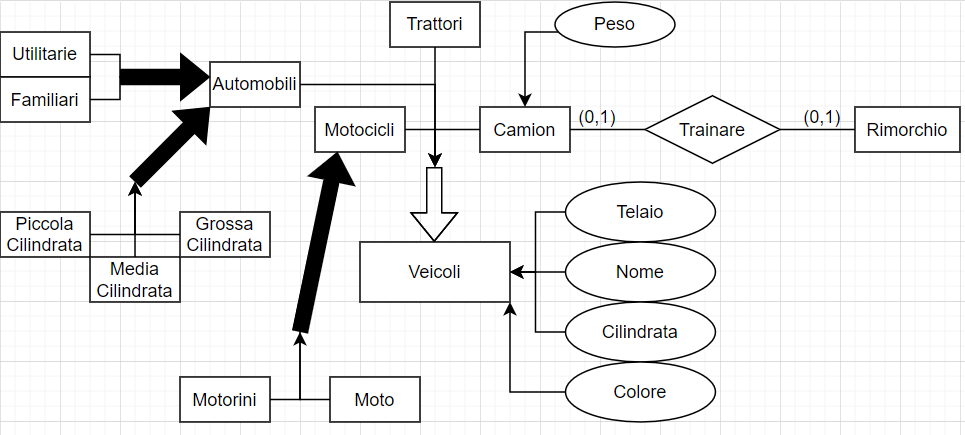
\includegraphics{Es2.png}}
\caption{\href{run:./TestoEs2.txt}{Testo dell'esercizio 2}}
\label{fig}
\end{figure}


\end{document}
